\chapter{O modelo \textit{cross-and-bouquet}}

%O modelo \textit{cross-and-bouquet} usa CS para classificar imagens, no caso, dado um $frame$ encontrar a imagem em um dicionário mais parecida ele.

O modelo \textit{cross-and-bouquet} usa CS para classificar imagens, ou seja, dada uma amostra $y$ e uma família de imagens $(\Phi_i)$, encontrar qual $\Phi_i$ é mais próxima de $y$.

Podemos interpretar o problema $\eqref{eqn:P0}$ da seguinte forma: dado um vetor $y \in \mathbb{R}^m$, quais colunas $a_i \in \mathbb{R}^m$ de $A$ melhor representam $y$? Se $y$ puder ser escrito como $y = Ax$ com $x$ esparso, podemos assumir que a coluna $a_i$ mais próxima de $y$ é aquela onde $x_i$ possui maior valor absoluto, ou seja,

$$ i = \argmax_{j = 1, \hdots, n} \vert x_j \vert $$

%Dado um conjunto de sinais $a_i \in \mathbb{R}^m$ com $A = \left[ a_1 \vert \hdots \vert a_m]$ e uma amostra $y \in \mathbb{R}^m$
Como vimos, CS garante que conseguimos encontrar $x$ esparso resolvendo $\eqref{eqn:P1}$ apenas quando $A$ é incoerente. Em aplicações, como em processamento de imagens, os vetores $a_i$ não são ``muito diferentes'' entre si, por isso não podemos assumir que $A$ é incorente. Então formularemos o problema de uma forma um pouco diferente:

Dado $y \in \mathbb{R}^m$ e $A$ uma matriz $m \gg n$ (ou seja, o número de amostras é pequeno se comparado à dimensão de cada amostra),

\begin{equation}
\tag{$\tilde{P_1}$}
\min_{x \in \mathbb{R}^n} \Vert x \Vert_{1} + \Vert e \Vert_{1} \textit{ sujeito a } y = Ax + e
%\label{eqn:P1_tilde}
\end{equation}

o que é equivalente a encontrar um vetor $c = \left[ \begin{tabular}{c}
x \\
e
\end{tabular} \right]$, com $x \in \mathbb{R}^n$ e $e \in \mathbb{R}^m$, onde $c$ resolve o problema

\begin{equation}
\tag{$\tilde{P_1}$}
\min_{c \in \mathbb{R}^{n + m}} \Vert c \Vert_{1} \textit{ sujeito a } y = \left[ \begin{tabular}{c c} A &  I \end{tabular} \right] c
\label{eqn:P1_tilde}
\end{equation}

onde $I$ é a matriz identidade $m \times m$.

Como $I$ é incoerente, pois é ortonormal, e possui muito mais colunas que $A$, é razoável supor que $\left[\begin{tabular}{c c} A &  I \end{tabular} \right]$ também seja incoerente e, neste caso, a solução $c$ de $\eqref{eqn:P1_tilde}$ seria esparsa.

Identificamos a amostra $y$ com o vetor $a_i$ onde
$$i = \argmax_{i = 1, \hdots, n} \vert c_i \vert$$

Essa é a ideia do modelo \textit{cross-and-bouquet} \cite{wrima}. O modelo tem esse nome porque as colunas de $I$ são ortonormais, lembrando uma cruz e as colunas de $A$ estão próximas, lembrando um buquê, como mostra a Figura \ref{fig:cross_bouquet}.

\begin{figure}
\centering
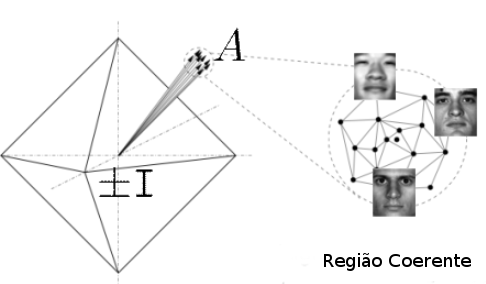
\includegraphics[scale=.6]{imagens/cross-and-bouquet.png}
\caption{Modelo \textit{cross-and-bouquet}. Imagem representando as colunas de $\left[ A \vert I \right]$ onde cada coluna de $A$ pode representar uma imagem, por exemplo. Adaptado de \cite{yangetal}.}
\label{fig:cross_bouquet}
\end{figure}